\documentclass[twoside]{article}
\setlength{\oddsidemargin}{0.25 in}
\setlength{\evensidemargin}{-0.25 in}
\setlength{\topmargin}{-0.6 in}
\setlength{\textwidth}{6.5 in}
\setlength{\textheight}{8.5 in}
\setlength{\headsep}{0.75 in}
\setlength{\parindent}{0 in}
\setlength{\parskip}{0.1 in}

\usepackage{graphicx}
\usepackage{url}
\usepackage{multicol}
\usepackage{listings}
\usepackage{float}

%
% The following commands sets up the lecnum (lecture number)
% counter and make various numbering schemes work relative
% to the lecture number.
%
\newcounter{lecnum}
\renewcommand{\thepage}{\thelecnum-\arabic{page}}
\renewcommand{\thesection}{\thelecnum.\arabic{section}}
\renewcommand{\theequation}{\thelecnum.\arabic{equation}}
\renewcommand{\thefigure}{\thelecnum.\arabic{figure}}
\renewcommand{\thetable}{\thelecnum.\arabic{table}}
\newcommand{\dnl}{\mbox{}\par}

%
% The following macro is used to generate the header.
%
\newcommand{\lecture}[4]{
  \pagestyle{myheadings}
  \thispagestyle{plain}
  \newpage
  \setcounter{lecnum}{#1}
  \setcounter{page}{1}
  \noindent
  \begin{center}
  \framebox{
     \vbox{\vspace{2mm}
   \hbox to 6.28in { {\bf CMPSCI~630~~~Systems
                       \hfill Fall 2014} }
      \vspace{4mm}
      \hbox to 6.28in { {\Large \hfill Lecture #1  \hfill} }
%       \hbox to 6.28in { {\Large \hfill Lecture #1: #2  \hfill} }
      \vspace{2mm}
      \hbox to 6.28in { {\it Lecturer: #3 \hfill Scribe: #4} }
     \vspace{2mm}}
  }
  \end{center}
  \markboth{Lecture #1: #2}{Lecture #1: #2}
  \vspace*{4mm}
}

%
% Convention for citations is authors' initials followed by the year.
% For example, to cite a paper by Leighton and Maggs you would type
% \cite{LM89}, and to cite a paper by Strassen you would type \cite{S69}.
% (To avoid bibliography problems, for now we redefine the \cite command.)
%
\renewcommand{\cite}[1]{[#1]}

% \input{epsf}

%Use this command for a figure; it puts a figure in wherever you want it.
%usage: \fig{NUMBER}{FIGURE-SIZE}{CAPTION}{FILENAME}
\newcommand{\fig}[4]{
           \vspace{0.2 in}
           \setlength{\epsfxsize}{#2}
           \centerline{\epsfbox{#4}}
           \begin{center}
           Figure \thelecnum.#1:~#3
           \end{center}
   }

% Use these for theorems, lemmas, proofs, etc.
\newtheorem{theorem}{Theorem}[lecnum]
\newtheorem{lemma}[theorem]{Lemma}
\newtheorem{proposition}[theorem]{Proposition}
\newtheorem{claim}[theorem]{Claim}
\newtheorem{corollary}[theorem]{Corollary}
\newtheorem{definition}[theorem]{Definition}
\newenvironment{proof}{{\bf Proof:}}{\hfill\rule{2mm}{2mm}}

% Some useful equation alignment commands, borrowed from TeX
\makeatletter
\def\eqalign#1{\,\vcenter{\openup\jot\m@th
 \ialign{\strut\hfil$\displaystyle{##}$&$\displaystyle{{}##}$\hfil
     \crcr#1\crcr}}\,}
\def\eqalignno#1{\displ@y \tabskip\@centering
 \halign to\displaywidth{\hfil$\displaystyle{##}$\tabskip\z@skip
   &$\displaystyle{{}##}$\hfil\tabskip\@centering
   &\llap{$##$}\tabskip\z@skip\crcr
   #1\crcr}}
\def\leqalignno#1{\displ@y \tabskip\@centering
 \halign to\displaywidth{\hfil$\displaystyle{##}$\tabskip\z@skip
   &$\displaystyle{{}##}$\hfil\tabskip\@centering
   &\kern-\displaywidth\rlap{$##$}\tabskip\displaywidth\crcr
   #1\crcr}}
\makeatother

% **** IF YOU WANT TO DEFINE ADDITIONAL MACROS FOR YOURSELF, PUT THEM HERE:



% Some general latex examples and examples making use of the
% macros follow.

\begin{document}

%FILL IN THE RIGHT INFO.
%\lecture{**LECTURE-NUMBER**}{**DATE**}{**LECTURER**}{**SCRIBE**}
\lecture{14}{October 30}{Emery Berger}{Amee Trivedi,Patrick Pegus}


\section*{Lecture Summary}
%\section{Summary}
\begin{itemize}
	\item Fail stop and Fail fast
	\item Air traffic control system
	\item Fault tolerance in web browser 
	\item Failure Oblivious computing
	\item Die Hard
\end{itemize}

\section{Fail stop and fail fast}

Fail stop means throw an exception when you detect failure
Fail fast means fail as soon as you detect failure

\section{Air traffic control system}
\begin{lstlisting}
		t1							t2
	if(runway[i] == empty){                 	if(runway[i] == empty){
	  runway[i] = flt1;				   runway[i] = flt25;
	} //OKAY to land				 } //OKAY to land
\end{lstlisting}

This could result in disaster because of possible race. So, to avoid this we can keep a count of the number of planes on the runway and then do an integrity check. If the integrity check fails, then, essentially,
the system throws an error. Humans catch the error by making phone calls and checking runways.
The airline traffic monitoring and control is basically a queuing system, it has a holding pattern where all the landing planes are queued and there is admissions control that creates the landing pressure. The other side of the system has takeoff queues that create back pressure. The holding pattern of the landing planes is basically the queue formed by planes circling above the airport at different heights and at different levels. In case of emergency the plane is redirected to another nearby airport for landing(Load shedding).

\begin{figure}[H]
\centering
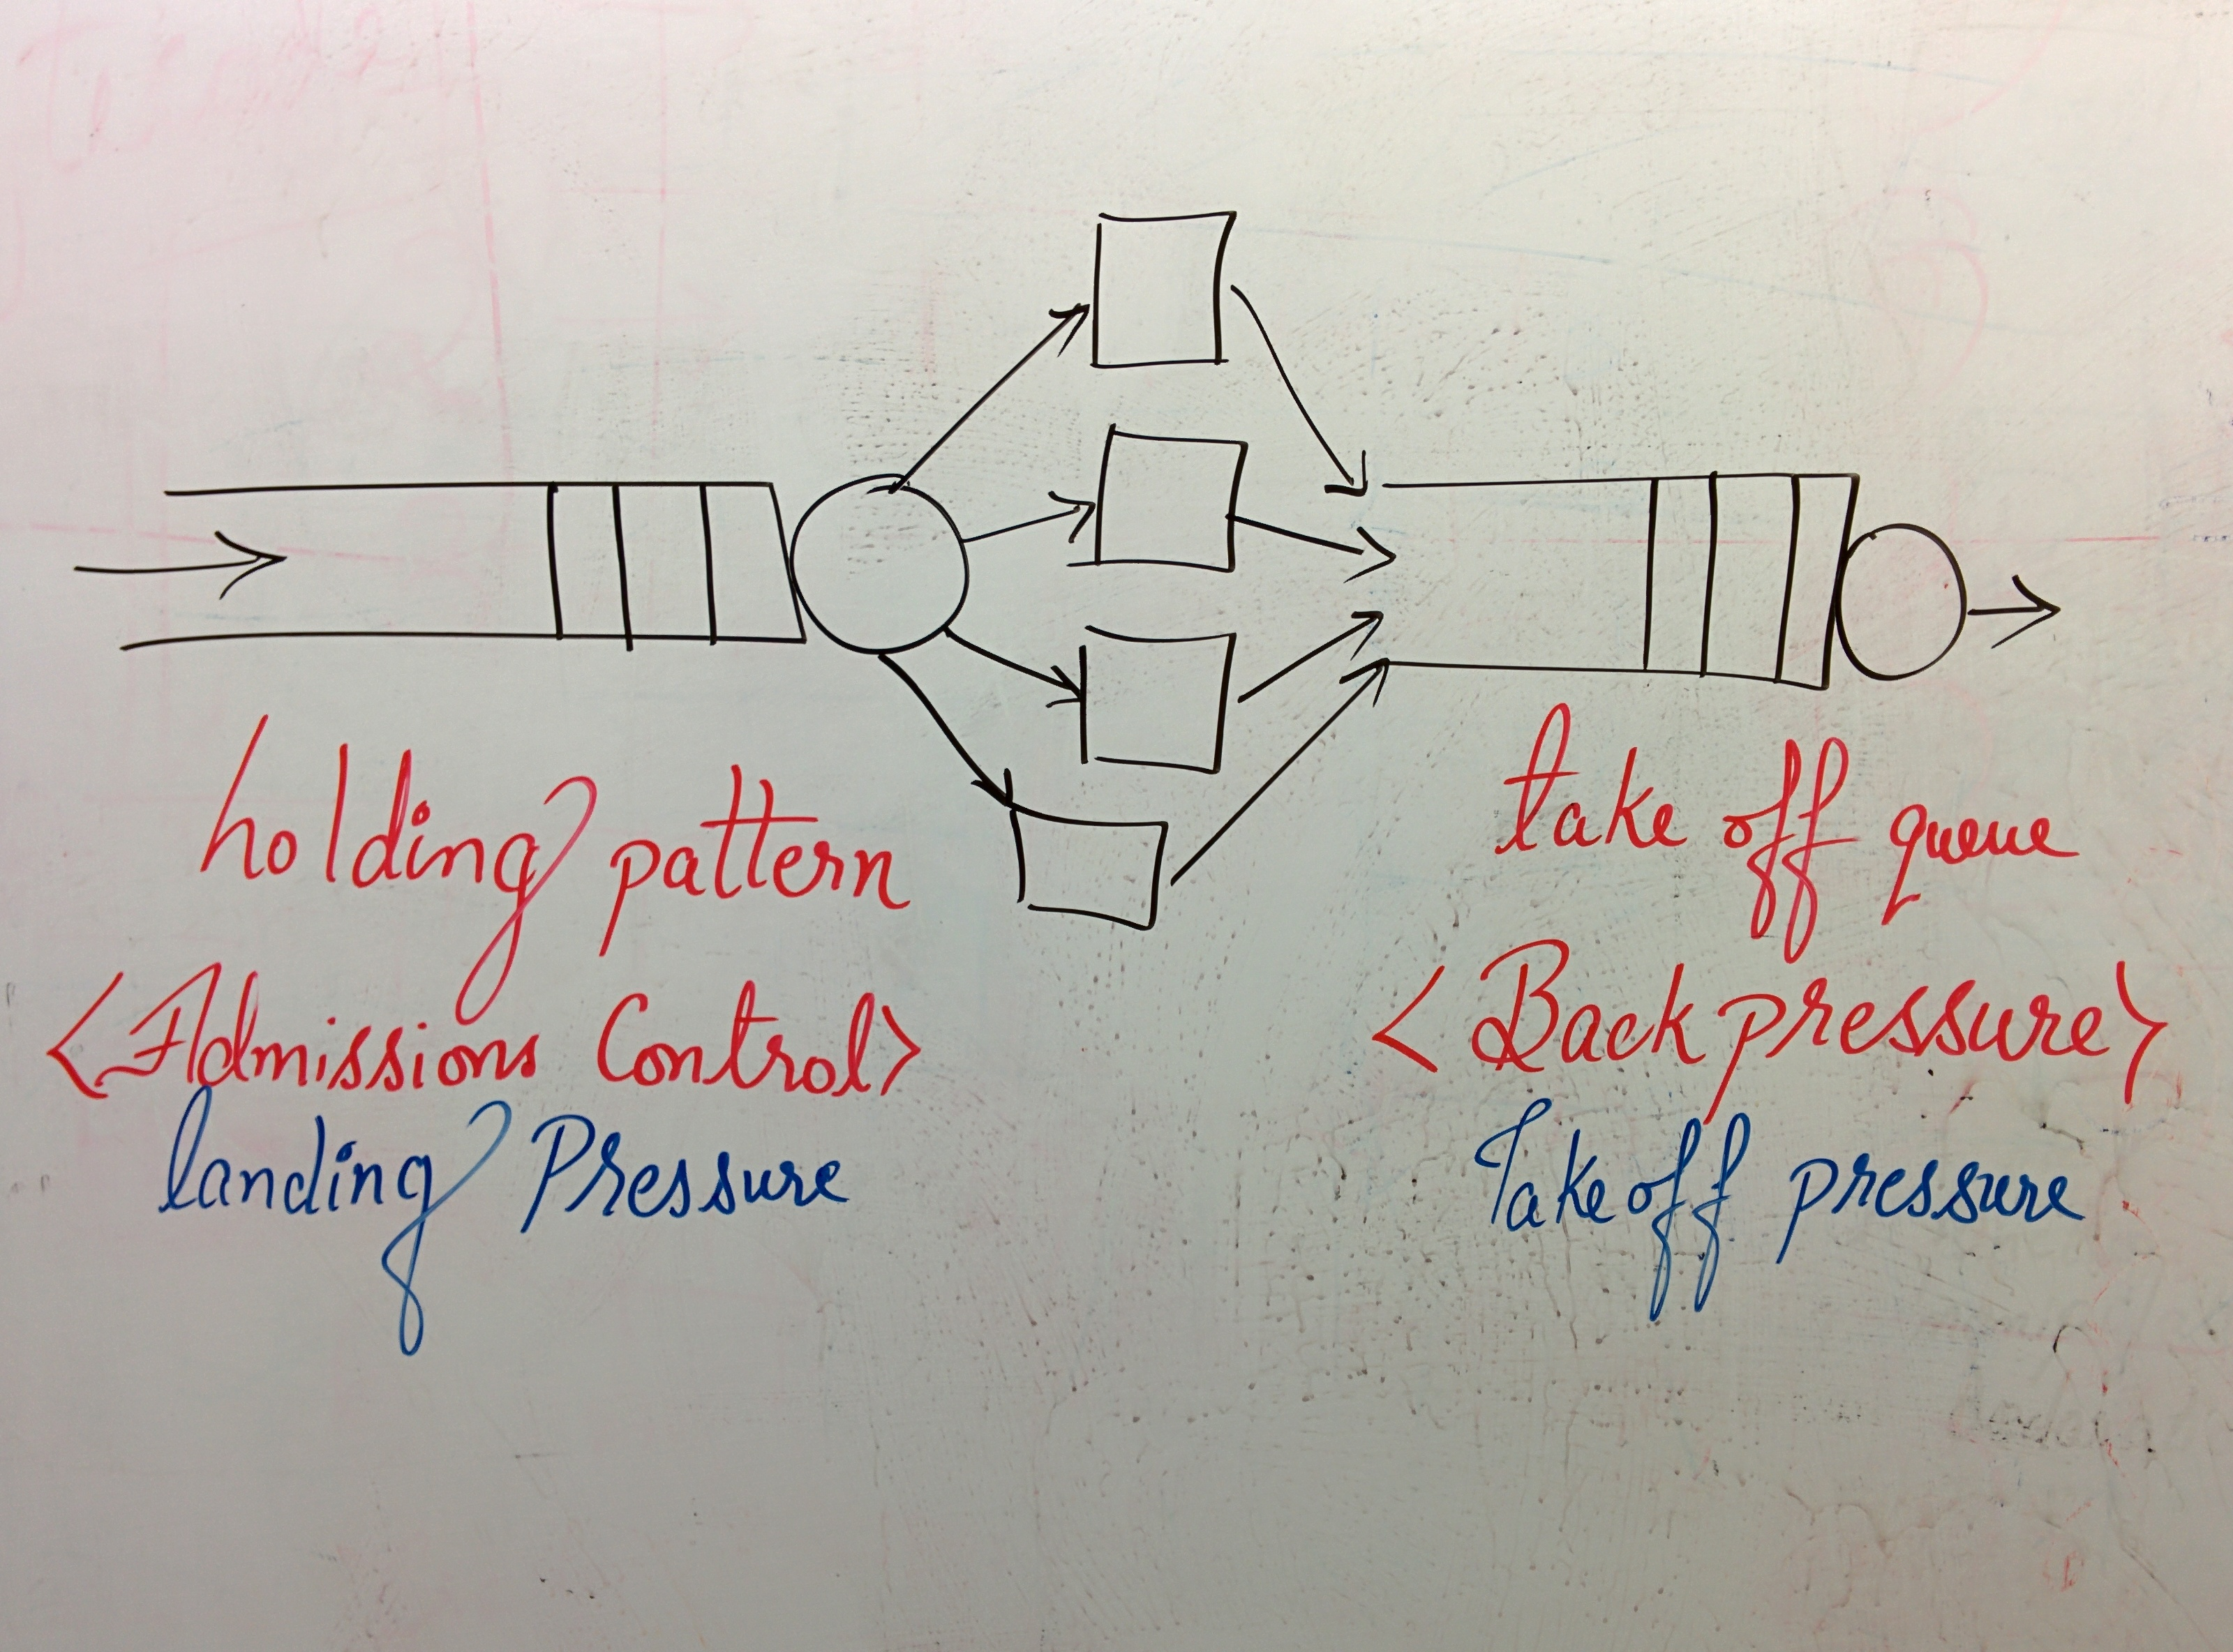
\includegraphics[width=150mm]{airplane_queue.jpg}
\caption{Flow diagram \label{Queuing Diagram}}
\end{figure}

\section{Tangent}
The difference between Airbus and Boeing is that Airbus flies mostly on automatic mode which is autopilot mode that is ON 99\% of the time. During that time, the pilot is only present to catch software exceptions. So, the fuel efficiency of Airbus is higher since the signals are sent to computer for interpretation and the computer decides the next action eg: change in altitude. Whereas a Boeing flight is manual. The pilots fly the plane resulting in higher fuel consumption.

In the Brazilian plane crash, a sensor iced over, which caused a software malfunction. The pilots could not correct this error due to low visibility.

With autopilot on the pilot is needed only during the take off time because wind sheer , what to do if a bird strikes or any other unpredictable events during takeoff cannot be handled by the computer. The autopilot is programmed in SCADE which generates C like code. It is not coded in C but in SCADE and then C code is generated because SCADE has no provision for dynamic memory allocation only static memory can be used, this reduces most of the errors.


\section{Fault tolerance in web browser}
Compared to the earlier scenario of an airplane a web browser has a very different approach to faults. Almost every web page has incorrect elements, however a web browser is not safety critical and its main purpose is to remain available. If fail stop is considered then availability pays the price and vice-versa. Hence, it allows errors and keeps loading the page. So, web browser tolerates failure by implementing the best effort approach.

\section{Failure Oblivious computing}
What should happen while executing the below code?

\begin{lstlisting}
	int x[100];
	x[200] = 12;
\end{lstlisting}
Given that in C it gives an undefined behaviour, what should be the behaviour of the system that executes the above code?

Answers:
1. 6 people said it should Fail
2. Amee said It depends, if the program is safety critical, the error impact is high or it gets propagated through the system then Fail else define a watermark for n errors to be allowed, once watermark is reached system panics.
3. Adam said give warnings stating "Bad Programmer" replace the instruction x[200] = 12 by NOP but for statements such as z = x[200] return a standard pre-defined value.
4. Ian said when x[200] is encountered extend the array. This would throw an exception in java. 
Other alternatives are to cache, write out of bounds, drop the value, lookup in cache or manufacture some value.

In Failure Oblivious Computing, it is difficult to determine the probability of errors.


\section{C Memory errors}
The main types of memory errors in C are:

\begin{itemize}
	\item Buffer Overflow : When allocated memory is too small and the write/assignment is for an index too far. Eg:
\begin{lstlisting}
	x = malloc(Too small)
	x[Too far]
\end{lstlisting}
This results in writing out of bounds.

	\item Dangling pointer : When you free something too soon.
\begin{lstlisting}
	p = malloc();
	free(p);
	p[0];
\end{lstlisting}
	\item Double free heap corruption:
		\begin{itemize}
			\item If the freelist, $F$, is implemented as a singly linked list, $free(X)$ adds a pointer, $p$, to $X$ pointing to the head of $F$. Then the pointer to $F$, $F*$, is changed
		to point to $X$. If that location is freed again, $p$ is updated to point to $X$ and $F*$ still points to $X$. Therefore, any calls to malloc return only $X$ and any change to a memory chunk subsequently returned by
		malloc is a change to all subsequently returned memory chunks, since they are all $X$.
			\item metadata corruption
		\end{itemize}
	\item uninitialized pointers
\end{itemize}

\section{DieHard}
In a system when you have infinite memory(infinite heap) then you can have infinite malloc's with infinite space between allocated memory, this is called infinite heap semantics.
But, since in real world it cannot be infinite so we approximate an infinite heap with a constant factor, $f$. DieHard uses a factor of 2. So, when allocation of $n$ bytes is requested, DieHard basically allocates a chunk
from a region that holds chunk sizes where $2^i-1<n<2^j$ and that region is less than $\frac{1}{f}$ allocated with uniform randomness over all such regions. That way, we can calculate the probability of corrupting memory,
which increases the farther we write outside of an allocated chunk.
It is implemented in Windows 7 as "fault tolerant heap" which can be set as the heap to be used by setting the crash velocity. If crash velocity = infinity it implies that a program will never switch to DieHard.

\end{document}
